\documentclass[12pt]{report}
\usepackage{graphicx}
\usepackage[utf8]{inputenc}
\usepackage[spanish]{babel}
\usepackage{setspace}
\usepackage{geometry}
\usepackage{titlesec}
\usepackage{times}
\usepackage{mathptmx} % Use mathptmx instead of times
\usepackage{fancyhdr}
\usepackage{float}
\usepackage{pdfpages}



% Configuración de márgenes
\geometry{
    top=2.5cm,
    left=3cm,
    right=3cm,
    bottom=2.5cm
}

% Configuración de interlineado
\onehalfspacing

% Configuración de títulos y subtítulos
\titleformat{\chapter}[display]
  {\normalfont\bfseries\centering}{}{0pt}{\fontsize{14}{16}\selectfont}
\titleformat{\section}
  {\normalfont\bfseries}{\thesection}{1em}{\fontsize{12}{14}\selectfont}
\titleformat{\subsection}
  {\normalfont\bfseries}{\thesubsection}{1em}{\fontsize{12}{14}\selectfont}


% Configuración de pie de página
  \fancyhf{}
\fancyfoot[R]{\thepage}
\pagestyle{fancy}
\fancypagestyle{plain}{
  \fancyhf{}
  \fancyfoot[R]{\thepage}
}

  \begin{document}
  \pagenumbering{roman}
%----- PORTADA ----
\setlength{\hoffset}{27 pt} % 1 (Para centrar más la portada)
\begin{titlepage}
{\centering
{\fontfamily{ptm}\scshape\bfseries\fontsize{29.16}{34.992}\selectfont Universidad de Guadalajara \par}
\vspace{0.5cm}
{\scshape\Large Centro Universitario de los Lagos \par}
\vspace{1cm}
{\scshape\Large División de Estudios de la Biodiversidad e innovación Tecnológica \par}
\vspace{1cm}
{\graphicspath{{imagenes/Portada}} %ruta de las imagenes

\includegraphics[width=0.3\textwidth]{image.png}\par}
\vspace{1cm}
% Título
{\scshape\large\bfseries Practica 7: Semaforo en cruce de dos calles\par}
\vspace{0.5cm}
% Materia
{\large \textbf{Materia:} \\Controladores Lógicos Programables\par}
\vfill
% Estudiante
{\large \textbf{Presenta:} \\Oscar Iván Moreno Gutiérrez \#220942754
\\Maximiliano Frias Campos \#217488066
\par}
\vfill
% Profesor
{\large \textbf{Profesor:} \\Dr. Afanador Delgado Samuel Mardoqueo \par}
\vfill
\vfill
% Fecha
\begin{flushright}
  {\normalsize \textbf {Fecha:} \\ \today}
\end{flushright}
\vfill}
{\large  \par}
\end{titlepage}
%----- FIN DE PORTADA ----

%----- ÍNDICE GENERAL ----
\tableofcontents
\newpage

%----- PALABRAS CLAVE ----
\pagenumbering{arabic}
\chapter*{Palabras Clave}
  \begin{itemize}
    \item Semáforo: Dispositivo de señales luminosas para controlar el tráfico.
    \item Cruce de calles: Intersección donde se cruzan dos o más calles.
    \item Simulación: Imitación del funcionamiento de un sistema real.
    \item Controladores Lógicos Programables: Dispositivos electrónicos usados para automatizar procesos.
    \item Temporizadores: Dispositivos que miden y controlan intervalos de tiempo.
    \item Bobinas: Componentes electromagnéticos usados en circuitos.
  \end{itemize}
\addcontentsline{toc}{chapter}{Palabras Clave}


%\begin{itemize}

%\end{itemize}
\newpage

%----- OBJETIVO ----
\chapter*{Objetivo}
\addcontentsline{toc}{chapter}{Objetivo}
  Se realizo la simulacion de dos semaforos en un cruce de dos calles.
\newpage

%----- CONTENIDO ----
\chapter{Contenido}
\section{Problema a resolver}
  Se tiene la siguiente imagen del problema:
  \begin{figure}[H]
    \centering
    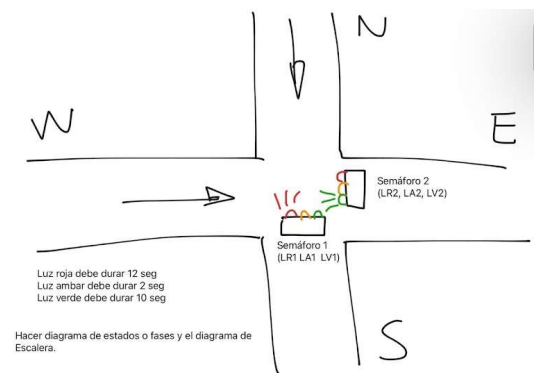
\includegraphics[width=0.5\textwidth]{screenshots/problema.png}
    \caption{Imagen del problema}
    \label{fig:imagen}
  \end{figure}
  Se puede observar que se tiene un cruce de dos calles, en donde se tiene un semaforo para cada calle. Se desea simular el funcionamiento de los semaforos,donde la luz verde dura 10 segundos, la luz amarilla 2 segundos y la luz roja 12 segundos.
\section{Como resolver el problema}
  Podemos deducir que habra 2 entradas:
  \begin{itemize}
    \item \textbf{Input 1:} Boton que inicia el circuito
    \item \textbf{Input 2:} Boton que detiene el circuito
  \end{itemize}
  Y habra 6 salidas por el total de luces de los semaforos:
  \begin{itemize}
    \item \textbf{Output 1:} Luz verde del semaforo 1
    \item \textbf{Output 2:} Luz amarilla del semaforo 1
    \item \textbf{Output 3:} Luz roja del semaforo 1
    \item \textbf{Output 4:} Luz verde del semaforo 2
    \item \textbf{Output 5:} Luz amarilla del semaforo 2
    \item \textbf{Output 6:} Luz roja del semaforo 2
  \end{itemize}
  Utilizaremos 7 bobinas para controlar el flujo de las luces de los semaforos , donde hay una bobina para cada luz de cada semaforo y una bobina para el boton de inicio.
  \begin{itemize}
    \item \textbf{Bobina 1:} Luz verde del semaforo 1
    \item \textbf{Bobina 2:} Luz amarilla del semaforo 1
    \item \textbf{Bobina 3:} Luz roja del semaforo 1
    \item \textbf{Bobina 4:} Luz verde del semaforo 2
    \item \textbf{Bobina 5:} Luz amarilla del semaforo 2
    \item \textbf{Bobina 6:} Luz roja del semaforo 2
    \item \textbf{Bobina 7:} Boton de inicio
  \end{itemize}
  Se pienza utilizar 13 temporizadores, ya que 12 de ellos se diviran en pareja para poder mandar un pulso al terminar el tiempo de una luz, pasando a la siguiente luz, y al mismo tiempo manteniendo la luz correspondiente encendida.
  El otro temporizador se utilizara para crear un pulso para encender los semaforos.
\section{Diagrama de Estados}


\section{Procedimiento}
\begin{enumerate}
  \item Declaramos las variables de nuestro circuito.
    \begin{figure}[H]
      \centering
      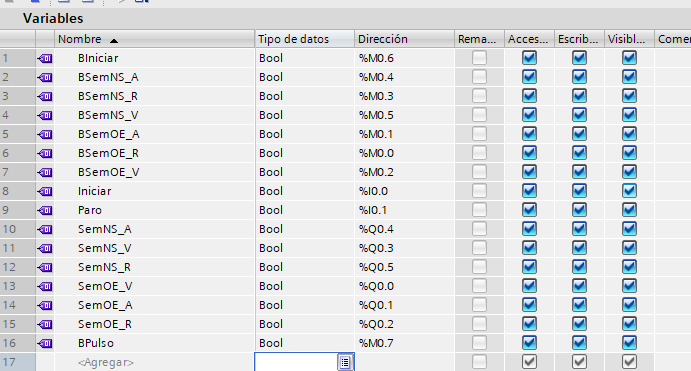
\includegraphics[width=0.5\textwidth]{screenshots/Variables.png}
      \caption{Variables del circuito}
      \label{fig:variables}
    \end{figure}
  \item Creamos el circuito


\end{enumerate}

\newpage
\begin{figure}[H]
  \centering
  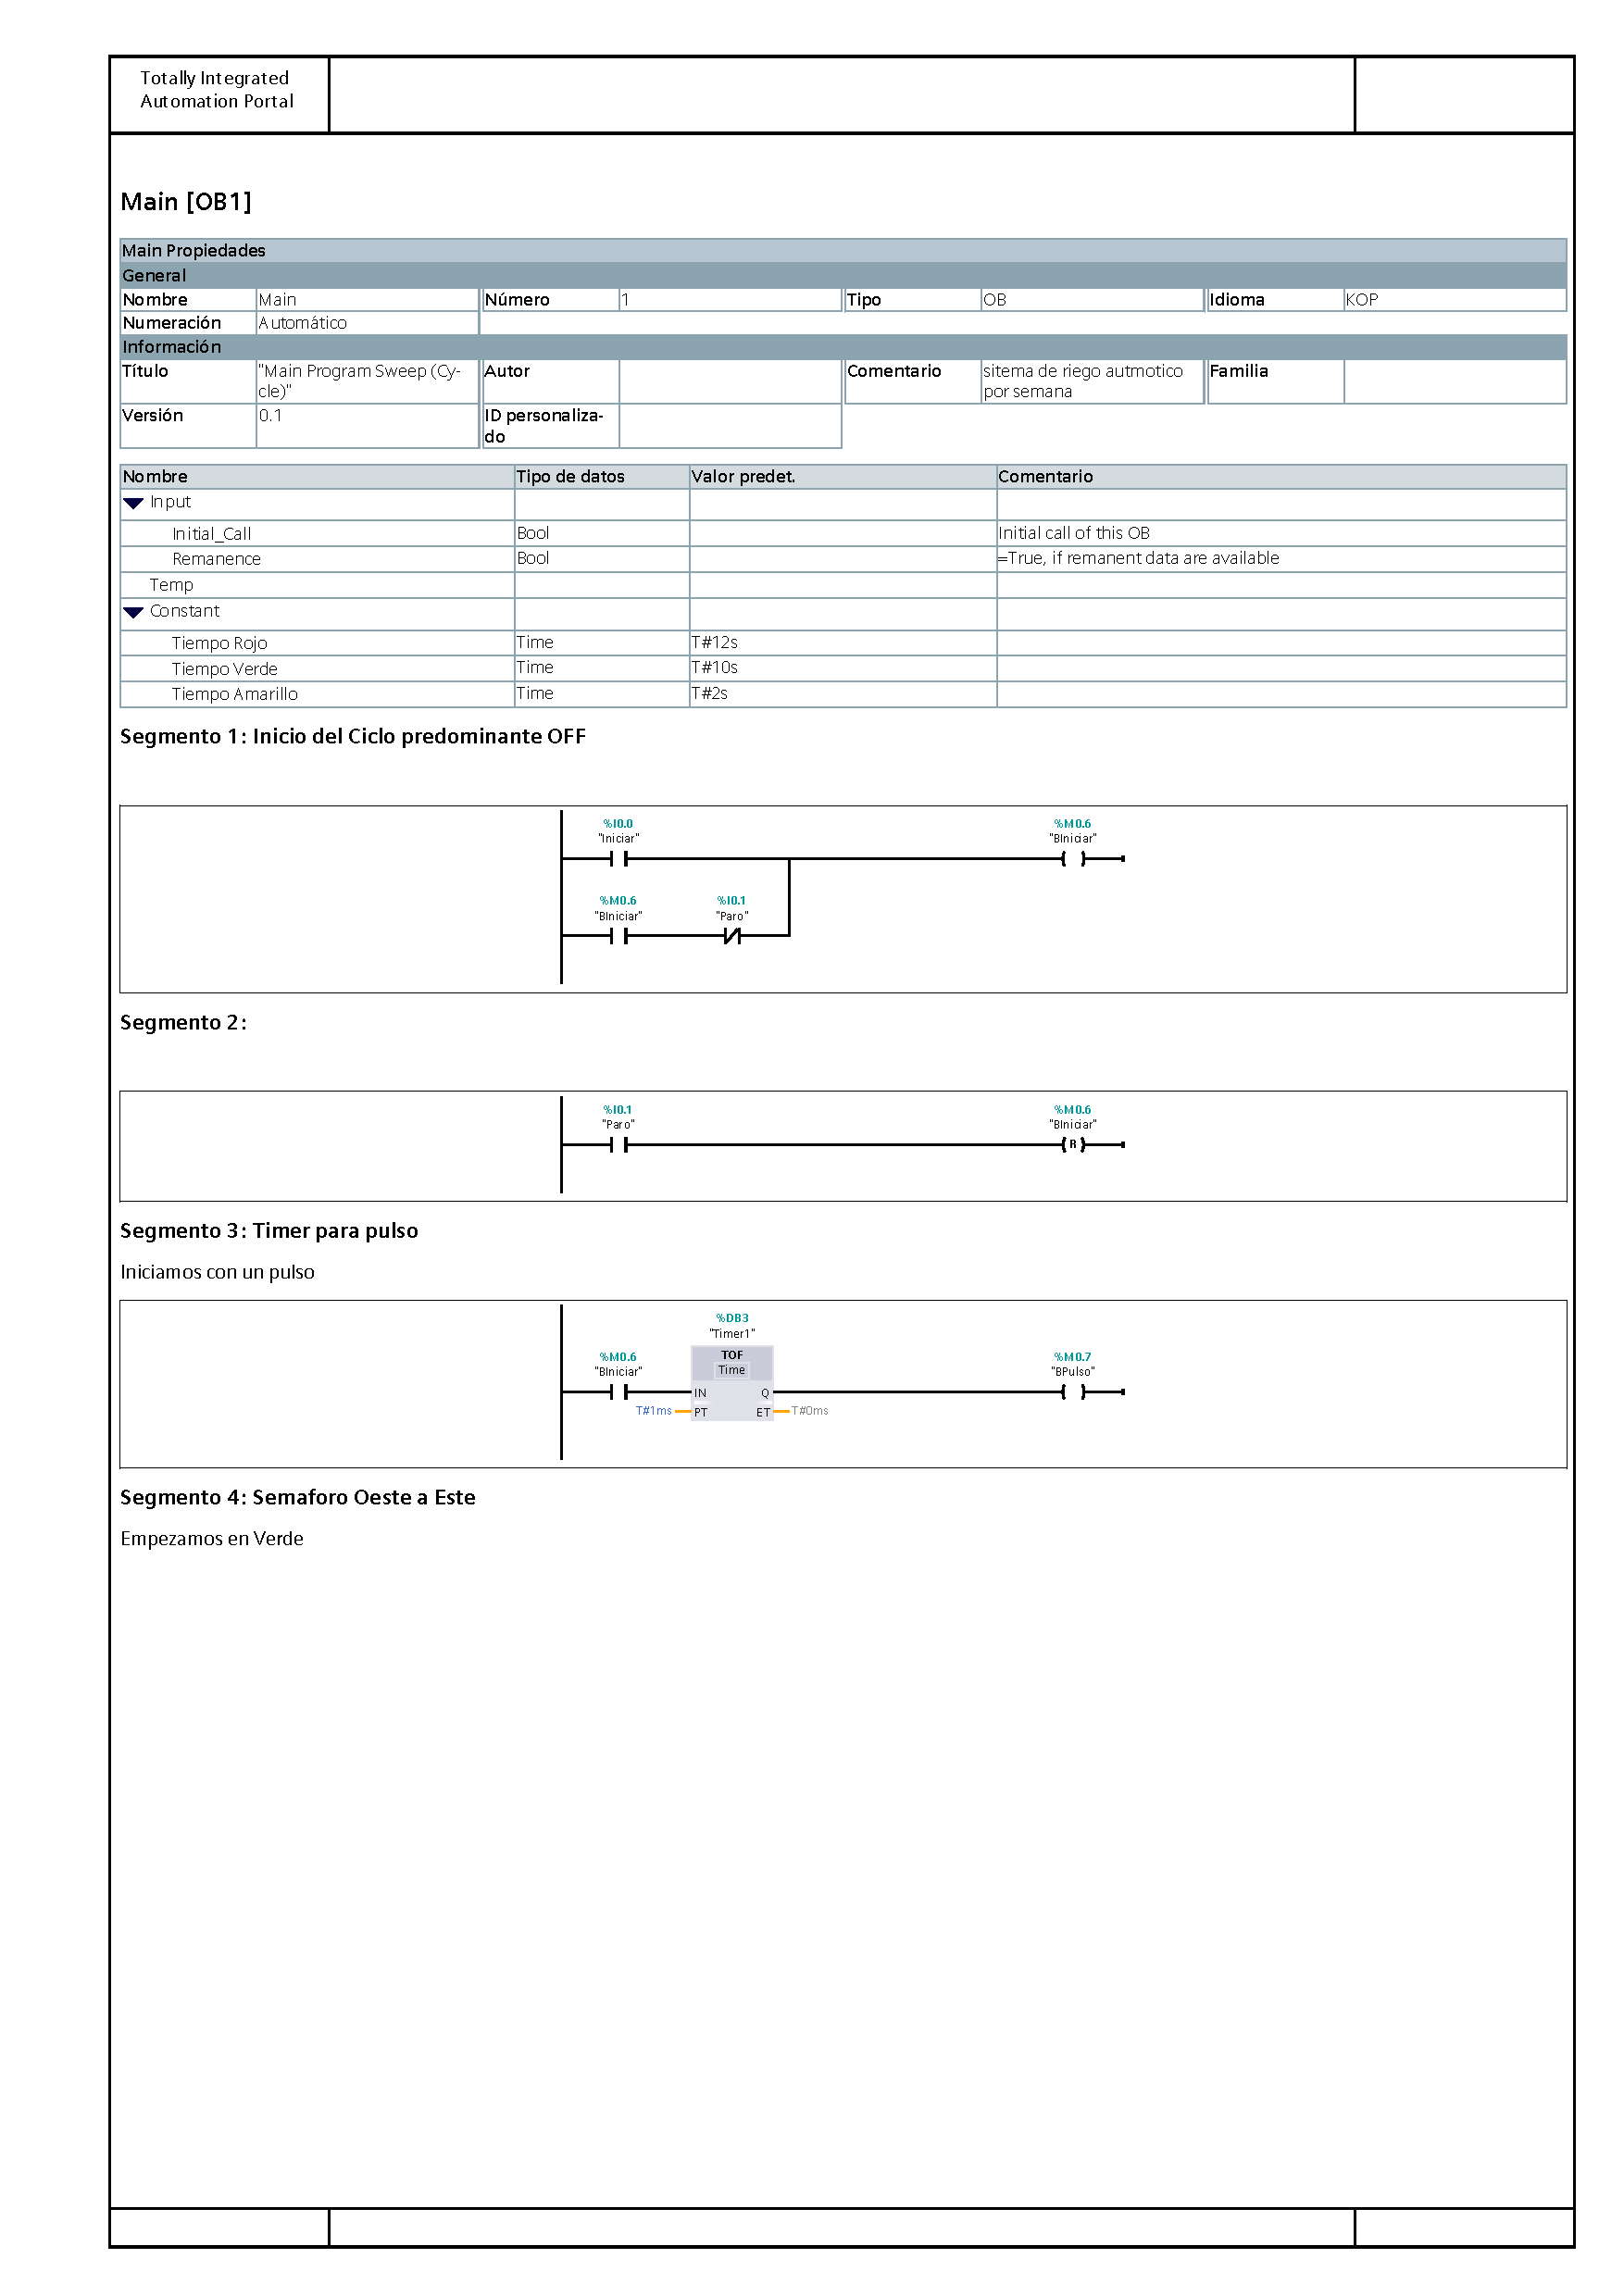
\includepdf[width=0.8\textwidth,page=1]{screenshots/P7.pdf} % Replace with the actual path to your PDF file
  \caption{circuito}
  \label{fig:pdfimage}
\end{figure}
\newpage

%----- CONCLUSIONES ----
\chapter{Conclusiones}
  Utilizando los temporizadores TOF y TON y unas cuantas bobinas pudimos crear este circuito.
\newpage


\end{document}